\section{Wave Parameters and Passive High-Frequency Components}
\begin{itemize}
    \itemsep0pt
    \item Scattering matrix $S$:
        \[\begin{bmatrix}b_1\\ b_2\end{bmatrix} =\
            \begin{bmatrix}S_{11} & S_{12}\\ S_{21} & S_{22}\end{bmatrix} \
            \begin{bmatrix}a_1\\ a_2\end{bmatrix}\]
            \item \textbf{Symmetry:} \(\left(S = S^\top\right) \land \left(S_{ii} = S_{jj}\;\;\forall\:i, j \in \left[1;\:\mathrm{dim}\{S\}\right]\,\right)\)
                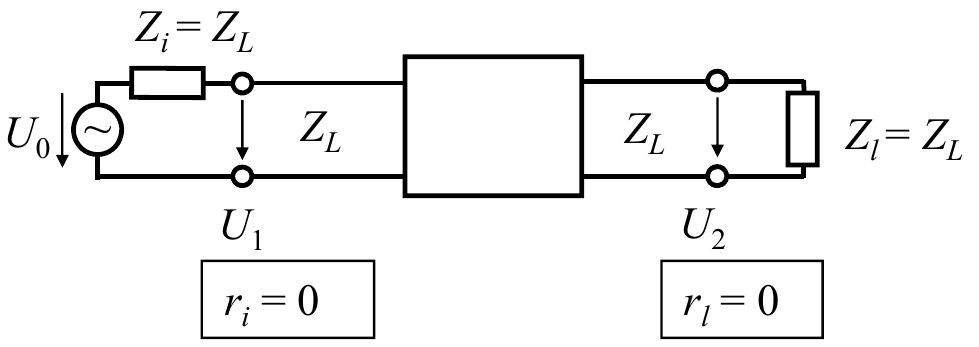
\includegraphics[width=.3\paperheight]{content/hfcomp/pictures/general_two-port.png}
    \item For a general 2-port, the following holds:
        \begin{flalign*}
            &S_{21} = 2 \dfrac{U_2}{U_0} \sqrt{\dfrac{Z_1}{Z_2}},\;\; S_{12} = 2 \dfrac{U_1}{U_0} \sqrt{\dfrac{Z_2}{Z_1}},\\
            &U_{f1} = \dfrac{U_0}{2},\;\; g_T = |S_{21}|^2,\;\; \dfrac{U_2}{U_1} = \dfrac{S_{21}}{(1 + S_{11})}
        \end{flalign*}
    \item For \(Z_{L1} \neq Z_{L2}\), all of the above equations hold, if $U_f$ and $U_b$ are replaced by \textit{normalized power wave amplitudes}:
        \begin{align*}
            &a_i = \dfrac{U_{fi}}{\sqrt{Z_{Li}}} &b_i = \dfrac{U_{bi}}{\sqrt{Z_{Li}}}
        \end{align*}
\end{itemize}

\subsection{Even/Odd Exitation of Symmetric Circuits}
\begin{itemize}
    \itemsep0pt
    \item Split a symmetric circuit into two less complex circuits
    \item \textit{Even(+)}-mode: in-phase excitation at both ports
    \item \textit{Odd(-)}-mode: excitation with opposite phases at both ports
    \item S-parameters of the original four-port are formally found to be:
        \begin{align*}
            S_{11} &= \dfrac{1}{2} (S_{11,e} + S_{11,o}),\\
            S_{21} &= \dfrac{1}{2} (S_{21,e} + S_{21,o}),\\
            S_{31} &= \dfrac{1}{2} (S_{21,e} - S_{21,o}),\\
            S_{41} &= \dfrac{1}{2} (S_{11,e} - S_{11,o}),\\
        \end{align*}
\end{itemize}

\subsection{Wilkinson Divider}
\begin{center}
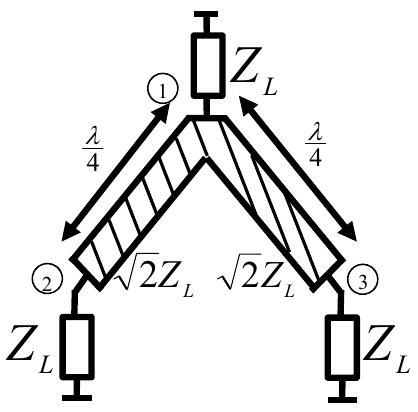
\includegraphics[width=3cm]{content/hfcomp/pictures/lossless_wilkinson_divider.png}
\end{center}
\begin{itemize}
    \itemsep0pt
    \item Input power is equally divided among the output ports, without reflections at the input port
    \item Scattering matrix with(-out) transverse resistor:
        \begin{align*}
            &\text{Without (lossless):} & S &= \
            \begin{bmatrix}\
                0 & \frac{-j}{\sqrt{2}} & \frac{-j}{\sqrt{2}}\\\
                \frac{-j}{\sqrt{2}} & \frac{1}{2} & \frac{-1}{2}\\\
                \frac{-j}{\sqrt{2}} & \frac{-1}{2} & \frac{1}{2}\
            \end{bmatrix}\\
            &\text{With (lossy):} & S &= \dfrac{-j}{\sqrt{2}}\
            \begin{bmatrix}\
                0 & 1 & 1\\\
                1 & 0 & 0\\\
                1 & 0 & 0\
            \end{bmatrix}\\
        \end{align*}
\end{itemize}

\subsection{Transmission Line Hybrid Coupler}
\begin{itemize}
    \itemsep0pt
    \item When \textit{fed at one port}, one output port is \textit{decoupled} and the other two output ports have \textit{equal amplitude}, but \textit{different phase differences} dependant on the design
    \item Most often: \ang{90}-hybrid, \ang{180}-hybrid Rat-Race
    \item Scattering matrix of \ang{90}-hybrid coupler with coupling factor $k$:
        \begin{align*}
            S &=
            \begin{bmatrix}\
                0 & k & -j\tau & 0\\\
                k & 0 & 0 & -j\tau\\\
                -j\tau & 0 & 0 & k\\\
                0 & -j\tau & k & 0\
            \end{bmatrix}\\
            \tau &= \sqrt{1 - k^2}
        \end{align*}
\end{itemize}

\subsection{Coupled Transmission Lines}
\begin{itemize}
    \itemsep0pt
    \item Unshielded transmission lines (in close proximity) are electromagnetically coupled $\implies$ directional couplers and bandpass filters can be realized
    \item Transmission line model with \textit{coupling capacitor} (elec. coupling) and \textit{coupling inductor} (magn. coupling)
%        \begin{align*}
%            &\frac{\mathrm{d}I_1}{\mathrm{d}z} = -j\omega(C^\prime_1 + C^\prime_{12})U_1 + j\omega C^\prime_{12}U_2\\
%            &\frac{\mathrm{d}I_2}{\mathrm{d}z} = -j\omega(C^\prime_2 + C^\prime_{12})U_2 + j\omega C^\prime_{12}U_1\\
%            &\frac{\mathrm{d}U_1}{\mathrm{d}z} = -j\omega L^\prime_1 I_1 - j\omega M^\prime I_2\\
%            &\frac{\mathrm{d}U_2}{\mathrm{d}z} = -j\omega L^\prime_2 I_2 - j\omega M^\prime I_1\\
%            &k = \frac{M^\prime}{L^\prime}\text{ (coupling coef.)}
%        \end{align*}
    \item For a transformer (inductive coupling):
        \begin{minipage}{.3\paperheight}
            \begin{circuitikz}[>=stealth, straight voltages, scale=.65, transform shape]
    \draw (0,0) node[transformer core, american](T){}
    %%Transformer primary side
    (T.A1) node[]{}
    +(-.5,0) node[ocirc]{} to[short, i=$I_1$] (T.A1)
    (T.A2) node[]{}
    +(-.5,0) node[ocirc]{} to[short] (T.A2)
    (T.A1)++(-.5,0) to[open, v=$U_1$] +(0,-2)
    %%Transformer secondary side
    (T.B1) node[]{}
    +(.5,0) node[ocirc]{} to[short, i^=$I_2$] (T.B1)
    (T.B2) node[]{}
    +(.5,0) node[ocirc]{} to[short] (T.B2)
    (T.B1)++(.5,0) to[open, v=$U_2$] +(0,-2);
    \draw [to-to] (T.inner dot A1) to[out=60, in=120] node[anchor=south]{$M$} (T.inner dot B1);
    \draw[-{Implies}, double, thick] (2,0) -- (2.5,0);
    \begin{scope}[xshift=7.5cm, yshift=0cm]
        \draw
        (0,0) node[transformer](G){}
        (G.A1) node[ocirc]{}
        to[short] +(-1,0)
        (G.A2) node[ocirc]{}
        to[short] +(-1,0)
        (G.B1) node[ocirc]{}
        (G.B2) node[ocirc]{};
        \path
        (G.inner dot A1) -- node[anchor=south]{$n:1$} (G.inner dot B1);
        \draw
        (G.A1)+(-1,0) to[L, *-*, american inductors, L=$k^2 L_1$]
        +(-1,-2.1);
        \draw
        (G.A1)++(-1,0) to[L, american inductors, L=$(1-k^2)L_1$] +(-2.5,0) node[ocirc]{}
        +(0,-2.1) to[short] +(-2.5,-2.1) node[ocirc]{};
%        ++(0,-2) to[short]
%        ++(-2,0) node[ocirc]{};
    \end{scope}
\end{circuitikz}

        \end{minipage}
        \begin{align*}
            &n = \dfrac{M}{L_2}, \quad k = \dfrac{M}{\sqrt{L_1 L_2}}\text{ (coupl. coeff.)},\\
            &\begin{bmatrix}\
                U_1\\
                I_1
            \end{bmatrix}\
            =\
            \begin{bmatrix}\
                n & 0\\
                0 & 1/n
            \end{bmatrix}\
            \begin{bmatrix}\
                U_2\\
                -I_2
            \end{bmatrix} \parbox{2cm}{(ideal trafo)}\\
            &L_1\text{: primary coil inductance}\\
            &L_2\text{: secondary coil inductance}
        \end{align*}
\end{itemize}

\subsection{Signal Flow Graphs}
\begin{itemize}
    \itemsep0pt
    \item Connection of wave amplitudes ($U_f$, $U_b$, $a$, $b$) by \textit{symbolic graph representation}
    \item \textbf{Vertex (knot):} wave amplitude
    \item \textbf{Branch:} transmission coefficient $S_{ij}$
    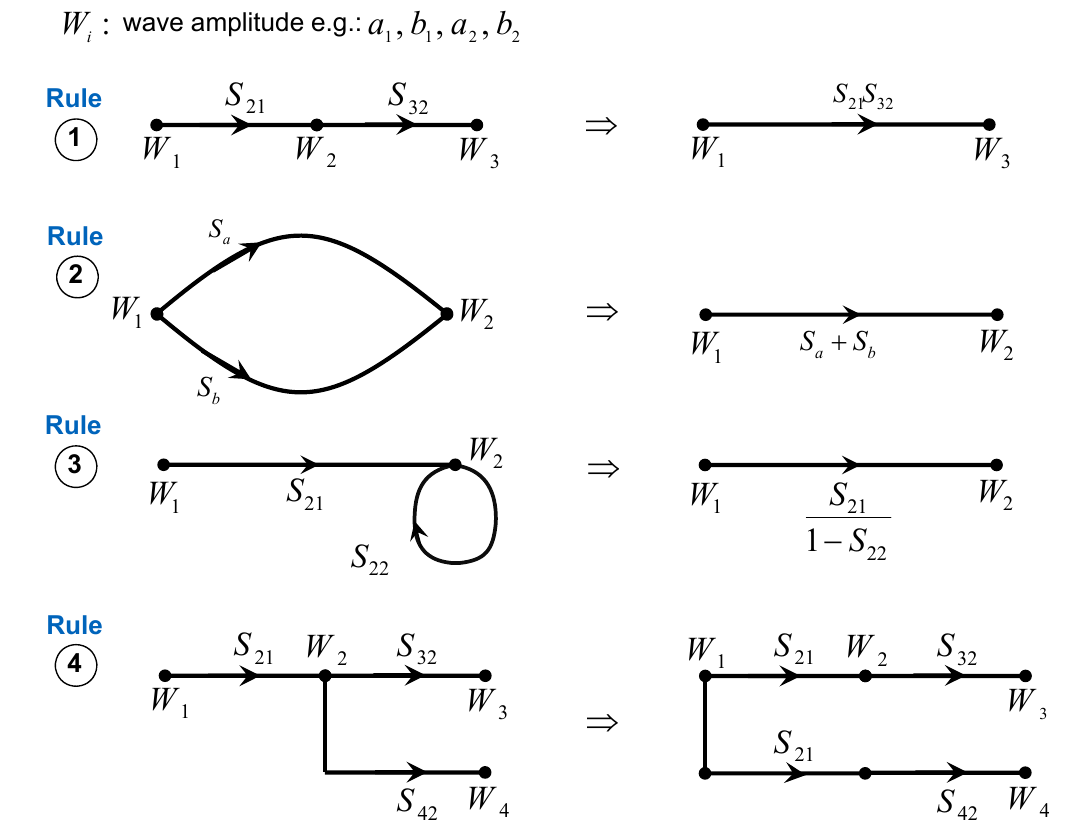
\includegraphics[width=.3\paperheight]{content/hfcomp/pictures/rules_signal_flow_graph.png}
    \item \textbf{Simplification rules for signal flow graphs:}
        \begin{enumerate}
            \item \(W_3 = S_{21}S_{32} W_1\)
            \item \(W_2 = W_1 S_a + W_1 S_b\)
            \item \(W_2 = W_1 \dfrac{S_{21}}{1 - S_{22}}\)
            \item Signal flow must not be changed!!!
        \end{enumerate}
    \item Analysis by Mason's Gain Rule:
        \begin{itemize}
            \itemsep0pt
%            \item \textbf{Independant variable:} Vertex of incident wave ($U_{fi}$, $a_i$)
%            \item \textbf{Dependant variable:} Vertex of an outgoing wave ($U_{bi}$, $b_i$)
            \item \textbf{Path:} Propagation path from an independant vertex ($a_i$) to a dependant vertex ($b_i$)following the positive direction of the branches, such that no vertex is passed more often than once.
            \item \textbf{Path Value:} Product of the branch coefficients of all branches along the path.
            \item \textbf{Loop of first order $L(1)$:} Product of the branch coefficients on a closed loop from one vertex back to the same vertex without passing any vertex twice.
            \item \textbf{Loop of second order $L(2)$:} Product of \textit{two loops of first order}, which do not touch (not even in a vertex).
            \item \textbf{Loop of third order $L(3)$:} Product of \textit{three loops of first order}, which do not touch (not even in a vertex).
            \item \textbf{Mason's Gain Rule:}
                \begin{align*}
                    &T = \dfrac{P_1 \xi_1 + P_2\xi_2 + P_3\xi_3 +...}{1 - \sum L(1) + \sum L(2) - \sum L(3) + ...},\\\\
                    &\xi_i = \left(1 - \sum L(1)^i + \sum L(2)^i - ...\right),\\
                    &L(1)^i:\parbox{4cm}{loops of order 1 that don't touch path $P_i$}
                \end{align*}
        \end{itemize}
\end{itemize}

\subsection{Non-Reciprocal Ferrite  Components}
\begin{itemize}
    \itemsep0pt
    \item In general: \(\mu_r = \mu_r^\prime - j\mu''_r\)
    \item YIG-Filter ($Y_3 Fe_2 O_{12}$) $\implies$ $H_0$ controls filter behaviour; selectively choose for left-/right-handed polarization
    \item \textit{Faraday Rotation} due to different permeabilites for left-/right-handed circ. pol. waves due to gyro-magnetic effects
    \item Uni-line circulator uses Faraday rotation to realize \textit{one-way} transmission line
    \item Y-Circulator (3-port) used to decouple transmitter-antenna-receiver for high powers
\end{itemize}
